% This is samplepaper.tex, a sample chapter demonstrating the
% LLNCS macro package for Springer Computer Science proceedings;
% Version 2.20 of 2017/10/04
%
\documentclass[runningheads]{llncs}
%
\usepackage{graphicx}
% Used for displaying a sample figure. If possible, figure files should
% be included in EPS format.
%
% If you use the hyperref package, please uncomment the following line
% to display URLs in blue roman font according to Springer's eBook style:
% \renewcommand\UrlFont{\color{blue}\rmfamily}
\usepackage{amsmath}

\begin{document}
%
\title{Deep Triplet Network adopting the Kernel and the Range Space Learning for Wi-Fi Handwritten Signature Verification}
%
\titlerunning{Triplet Network adopting KAR Learning for Wi-Fi Signature Verification}
% If the paper title is too long for the running head, you can set
% an abbreviated paper title here
%
\author{Young-Woong Kwon \and Jooyoung Kim \and Kar-Ann Toh}
%
\authorrunning{Y. Kwon et al.}
% First names are abbreviated in the running head.
% If there are more than two authors, 'et al.' is used.
%
\institute{
School of Electrical and Electronic Engineering, Yonsei University, 50 Yonsei-ro, Seodaemun-gu, Seoul 03722, Republic of Korea\\
\email{\{herokwon, harrykim, katoh\}@yonsei.ac.kr}}
%
\maketitle              % typeset the header of the contribution
%
\begin{abstract}
%The abstract should briefly summarize the contents of the paper in 15--250 words.
In this paper, we propose an identity verification system based on the handwritten signature signals captured by the Wi-Fi CSI signal using triplet network. 
To refine the triplet inputs for the faster loss convergence, the kernel and the range space learning is adopted to mine the distinctive triple inputs from the training Wi-Fi signature signals. 
Subsequently, the triplet network utilizing the ConvNet structure is trained with the mined triplet inputs based on L-2 distance comparison. 
Our experiments on an in-house Wi-Fi handwritten signature signal dataset show encouraging verification accuracy with faster training loss convergence compare to the basic triplet network and the Siamese network.

\keywords{Wi-Fi signature signal \and in-air handwritten signature verification \and the Kernel and the Range space projection learning \and triplet network}
\end{abstract}
%
%
%
\section{Introduction}

In recent years, several behavioral biometric traits for identity authentication are investigated since they are free from the physical characteristic which user owns~\cite{bailador2011analysis}. Among the behavioral biometrics, the signature based user authentication~\cite{galbally2015line,sanmorino2012survey} is taking considerable interest with the development of the in-air signature recognition systems~\cite{galbally2015line,jeon2012system,malik20183dairsig}. 
With the help of sensors such as a depth camera~\cite{malik20183dairsig} or mobile sensor~\cite{jeon2012system}, the in-air signature recognition systems could have less spatial limitation in the signature acquisition process compare to other contact-based authentication systems. 

Recently, the commercial Wi-Fi device is also proposed to be utilized as a in-air signature acquisition sensor due to its easy accessible property \cite{moon2017air}. By capturing the Wi-Fi CSI signal to observe the distinctive motions, the Wi-Fi based in-air signature recognition system showed reasonable user verification performance~\cite{moon2017air}. However, the previous works on Wi-Fi signal based user authentication systems~\cite{hong2016wfid,moon2017air} utilized the conventional feature extraction method such as the Principal Components Analysis. Since the conventional feature extraction method is not enough to extract the direction- or pose-invariant features from the acquired in-air data, more recently, some studies attempted to implement the deep learning algorithms in Wi-Fi signal based user authentication systems for the better verification performance ~\cite{shi2017smart,pokkunuru2018neuralwave}. 

In this paper, we utilize the deep triplet network for identity verification based on Wi-Fi CSI signature signal. To achieve not only the promising verification accuracy but also the fast training loss convergence speed for the commercial use, we adopt the kernel and the range (KAR) space leaning~\cite{toh100,toh2018learning,toh2018analytic,toh2018gradient} to mine the distinctive triplet inputs for training the triplet network. Subsequently, the triplet network utilizing the ConvNet structure as a feature extractor is trained using the mined triplet inputs based on L-2 distance comparison.
The main contributions of our work can be summarized as follows:
\begin{itemize}
\item Proposal of a system for identity verification based on the Wi-Fi handwritten signature signals using deep triplet network.
\item Adopted the KAR space learning to mine the distinctive triplet inputs which boosted the convergence speed of the training loss in triplet network.
\item Provision of the experimental study on an in-house Wi-Fi handwritten signature signal dataset collected from 50 subjects.
\end{itemize}

The paper is organized as follows: the related works including triplet network and KAR space learning will be introduced in Section 2 for immediate reference. Our proposed method will be discussed in Section 3. Section 4 describes our experimental results and analysis. Some concluding remarks will be followed in Section 5.


\section{Related Works}

\subsection{Triplet Network}
A Triplet network is comprised of 3 instances of the same feedforward network (with shared parameters)\cite{hoffer2015deep}. It is widely used in face recognition \cite{schroff2015facenet} and person re-identification, which solves the matching problem of individuals and identity between camera images\cite{cheng2016person,chen2017beyond}.
The distinction between classes may be ambiguous in the above tasks since the targets may be looking in different directions or taking different positions.
to achieve good ability to distinguish between classes, a triplet network works by extract feature vectors which expand margins between same and different class. 

The loss function of triplet network is calculated as the difference in L-2 distance between anchor to each positive and negative triplet outputs.
Optimizing the training process is important because gradient vanishing can occur during training.
It happens when the negative class distance is much greater than positive class distance, the output of the loss function can down to zero as a result.
%Also, outliers in triplet input affects a lot to training since The loss function for triplet network depends on the distance between each triplet input.

There are many ways to optimize training. In \cite{schroff2015facenet}, selects inputs from large mini-batch at each training iteration using the network during training. \cite{cheng2016person} adds second margin for triplet loss to expand intra-class distance.
Following in \cite{chen2017beyond}, quadruplet loss function makes the distance between the same classes is less than the distance between any different classes. 

In this paper, we adopt multilayer feedforward networks trained by the kernel and the range space learning to select good triplet input for training the triplet network. It has advantage for reducing computing resources as well as boosting the training optimization.
% Rel works: KAR learning
\subsection{kernel and the range space learning}

Multilayer feedforward neural networks is widely known to be good for feature extractor and classifier.
This network is generally trained by the gradient descent method and backpropagation.
However, setting the learning parameters such as learning rate or momentum value is important to use the gradient descent method. 

%This training methods makes networks to fell into problems such as vanishing gradient or local minima.
%To avoid these problems, it is important to set the learning parameters such as learning rate or momentum value before training.

%Recently, according to \cite{guo2004pseudoinverse}, based on linear algebric method and pseudo-inverse, gradient-free learning methods is invented.
%Howeaver, network weights of the hidden layer has to be fixed as equal to the number of examples.

Recently, gradient-free learning framework based on series of kernel and range (KAR) space manipulation has developed \cite{toh2018learning,toh2018gradient}.
since it is trained by algebric methods, no learning parameters are needed to train the networks.
%there is no problems of vanishing gradient and local minima, 
using this novel framework, we can train multilayer feedforward neural networks with any numbers and size of layers.

% Karnet structure and mining samples.
Let the training dataset $\mathbf{X}\in{\mathrm{R}}^{m \times (n+1)}$ and $\mathbf{G}\in{\mathrm{R}}^{m \times n}$ is network outputs.
Multilayer neural network structure is shown below:

\begin{equation}
    \mathbf{G} = \sigma\left(\left[\mathbf{1},\sigma\left(\dots\left[\mathbf{1},\sigma\left(\left[\mathbf{1},\sigma\left(\mathbf{X}\mathbf{W}_{1}\right)\right]\mathbf{W}_{2}\right)\right]\dots\mathbf{W}_{(i-1)}\right)\right]\mathbf{W}_{i}\right),
\end{equation}
where $\mathbf{W}_{1}\in{\mathrm{R}}^{(n+1) \times h_{1}}$,$\mathbf{W}_{2}\in{\mathrm{R}}^{(h_{1}+1) \times h_{2}}$,$\dots,\mathbf{W}_{i}\in{\mathrm{R}}^{(h_{(i-1)}+1) \times n}$,$\mathbf{1}=\left[1,\dots,1\right]^{T}\\
\in{\mathrm{R}}^{m \times 1}$ and $\sigma(.)$ is activation function.

When all weights have been learned, for given anchor signal, hard negative samples can be mined among the distance of network output of desired signal $\mathbf{G}$ is below the threshold.

% training KARnet
Network learning is archived using one-hot encoded target $\mathbf{Y}\in{\mathrm{R}}^{m \times n}$ instead of network output $\mathbf{G}$.
After that, we have the weight matrix $\mathbf{W}_{1}\dots\mathbf{W}_{i}$ to train. the weight matrix can be separated into weights and bias term as
$\mathbf{W}_{2}\dots\mathbf{W}_{i}$ = 
$\begin{bmatrix}
\mathbf{w}_{2}^{T}\\\mathnormal{W}_{2}
\end{bmatrix}
\dots
\begin{bmatrix}
\mathbf{w}_{i}^{T}\\\mathnormal{W}_{i}
\end{bmatrix}$.

after assign random weights to $\mathbf{W}_{1}\dots\mathbf{W}_{i}$ , we get $\mathbf{W}_{1}$. it is solved as follows:

\begin{equation*}
    \left[\sigma^{-1}\left(\mathbf{Y}\right)-\mathbf{1}\cdot\mathbf{w}_{i}^{T}\right]\mathnormal{W}_{i}^\dagger = 
    \sigma\left(\dots\left[\mathbf{1},\sigma\left(\left[\mathbf{1},\sigma\left(\mathbf{X}\mathbf{W}_{1}\right)\right]\mathbf{W}_{2}\right)\right]\dots\mathbf{W}_{(i-1)}\right)
\end{equation*}
\begin{equation*}
    \begin{aligned}
        \Rightarrow
        \biggl[\sigma^{-1}\biggl(
        \dots
        \biggl[\sigma^{-1}\biggl(
            \left[\sigma^{-1}\left(\mathbf{Y}\right)-\mathbf{1}\cdot\mathbf{w}_{i}^{T}\right]\mathnormal{W}_{i}^\dagger
        \biggr)
        - \mathbf{1}\cdot\mathbf{w}_{(i-1)}^{T}\biggr]\mathnormal{W}_{(i-1)}^{\dagger}
        \dots\biggr)\\
        - \mathbf{1}\cdot\mathbf{w}_{2}^{T}\biggr]\mathnormal{W}_{2}^{\dagger} 
        = \sigma\left(\mathbf{X}\mathbf{W}_{1}\right)
    \end{aligned}
\end{equation*}
\begin{equation}
    \begin{aligned}
        \Rightarrow
        \mathbf{X}^{\dagger}\sigma^{-1}\biggl(
        \biggl[\sigma^{-1}\biggl(
        \dots
        \biggl[\sigma^{-1}\biggl(
            \left[\sigma^{-1}\left(\mathbf{Y}\right)-\mathbf{1}\cdot\mathbf{w}_{i}^{T}\right]\mathnormal{W}_{i}^\dagger
        \biggr)
        - \mathbf{1}\cdot\mathbf{w}_{(i-1)}^{T}\biggr]\mathnormal{W}_{(i-1)}^{\dagger}
        \dots\biggr)\\
        - \mathbf{1}\cdot\mathbf{w}_{2}^{T}\biggr]\mathnormal{W}_{2}^{\dagger}
        = \mathbf{W}_{1} .
    \end{aligned}
\end{equation}

After deriving the $\mathbf{W}_{1}$, the $\mathbf{W}_{2}$ also can be optimized as:

%\begin{multline*}
\begin{equation}
    \begin{aligned}
        \Rightarrow
        \left(\sigma\left(\mathbf{X}\mathbf{W}_{1}\right)\right)^{\dagger}
        \biggl(\dots
        \biggl[\sigma^{-1}\biggl(
            \left[\sigma^{-1}\left(\mathbf{Y}\right)-\mathbf{1}\cdot\mathbf{w}_{i}^{T}\right]\mathnormal{W}_{i}^\dagger
        \biggr)
        - \mathbf{1}\cdot\mathbf{w}_{(i-1)}^{T}\biggr]\mathnormal{W}_{(i-1)}^{\dagger}
        \dots\biggr)\\
        = \mathbf{W}_{2} .
    \end{aligned}
\end{equation}
%\end{multline*}

By repeating this process recursively until all weight matrix values are obtained, the $\mathbf{W}_{i}$ can be obtained as follows:
\begin{equation}
    \mathbf{W}_{i} = \left[\mathbf{1},\sigma\left(\dots\left[\mathbf{1},\sigma\left(\left[\mathbf{1},\sigma\left(\mathbf{X}\mathbf{W}_{1}\right)\right]\mathbf{W}_{2}\right)\right]\dots\mathbf{W}_{(i-1)}\right)\right]^{\dagger}\sigma^{-1}\left(\mathbf{Y}\right).
\end{equation}


%% Methods
\section{Proposed System}

% Methods: System overview(Fig.1)
In this section, we propose an identify verification system based on the Wi-Fi based in-air handwritten signature (will be called Wi-Fi signature signals hereafter). An overview of the proposed system utilizing the ConvNet \cite{lecun1998gradient} and the kernel and the range space projection learning (KAR space learning) \cite{toh2018learning,toh2018gradient} is shown in Fig.1.

Essentially, the Wi-Fi signature signals are randomly divided to create the training and the validation set. Subsequently, the KAR space projection learning generates the triplet data by mining the hard positve and the hard negative samples for the given anchor signal from the training dataset.

To train the ConvNet structure, generated triplet data flows into the predifined ConvNet structure. The ConvNet extracts feature vectors from given triplet input.
ConvNet training is achieved by the triplet loss, which is formulated by the L-2 distance metrics of feature vectors. The overall ConvNet network is trained by the backpropagation scheme. The following subsections detail the each step of the proposed system.

% Figure 1
\begin{figure}
    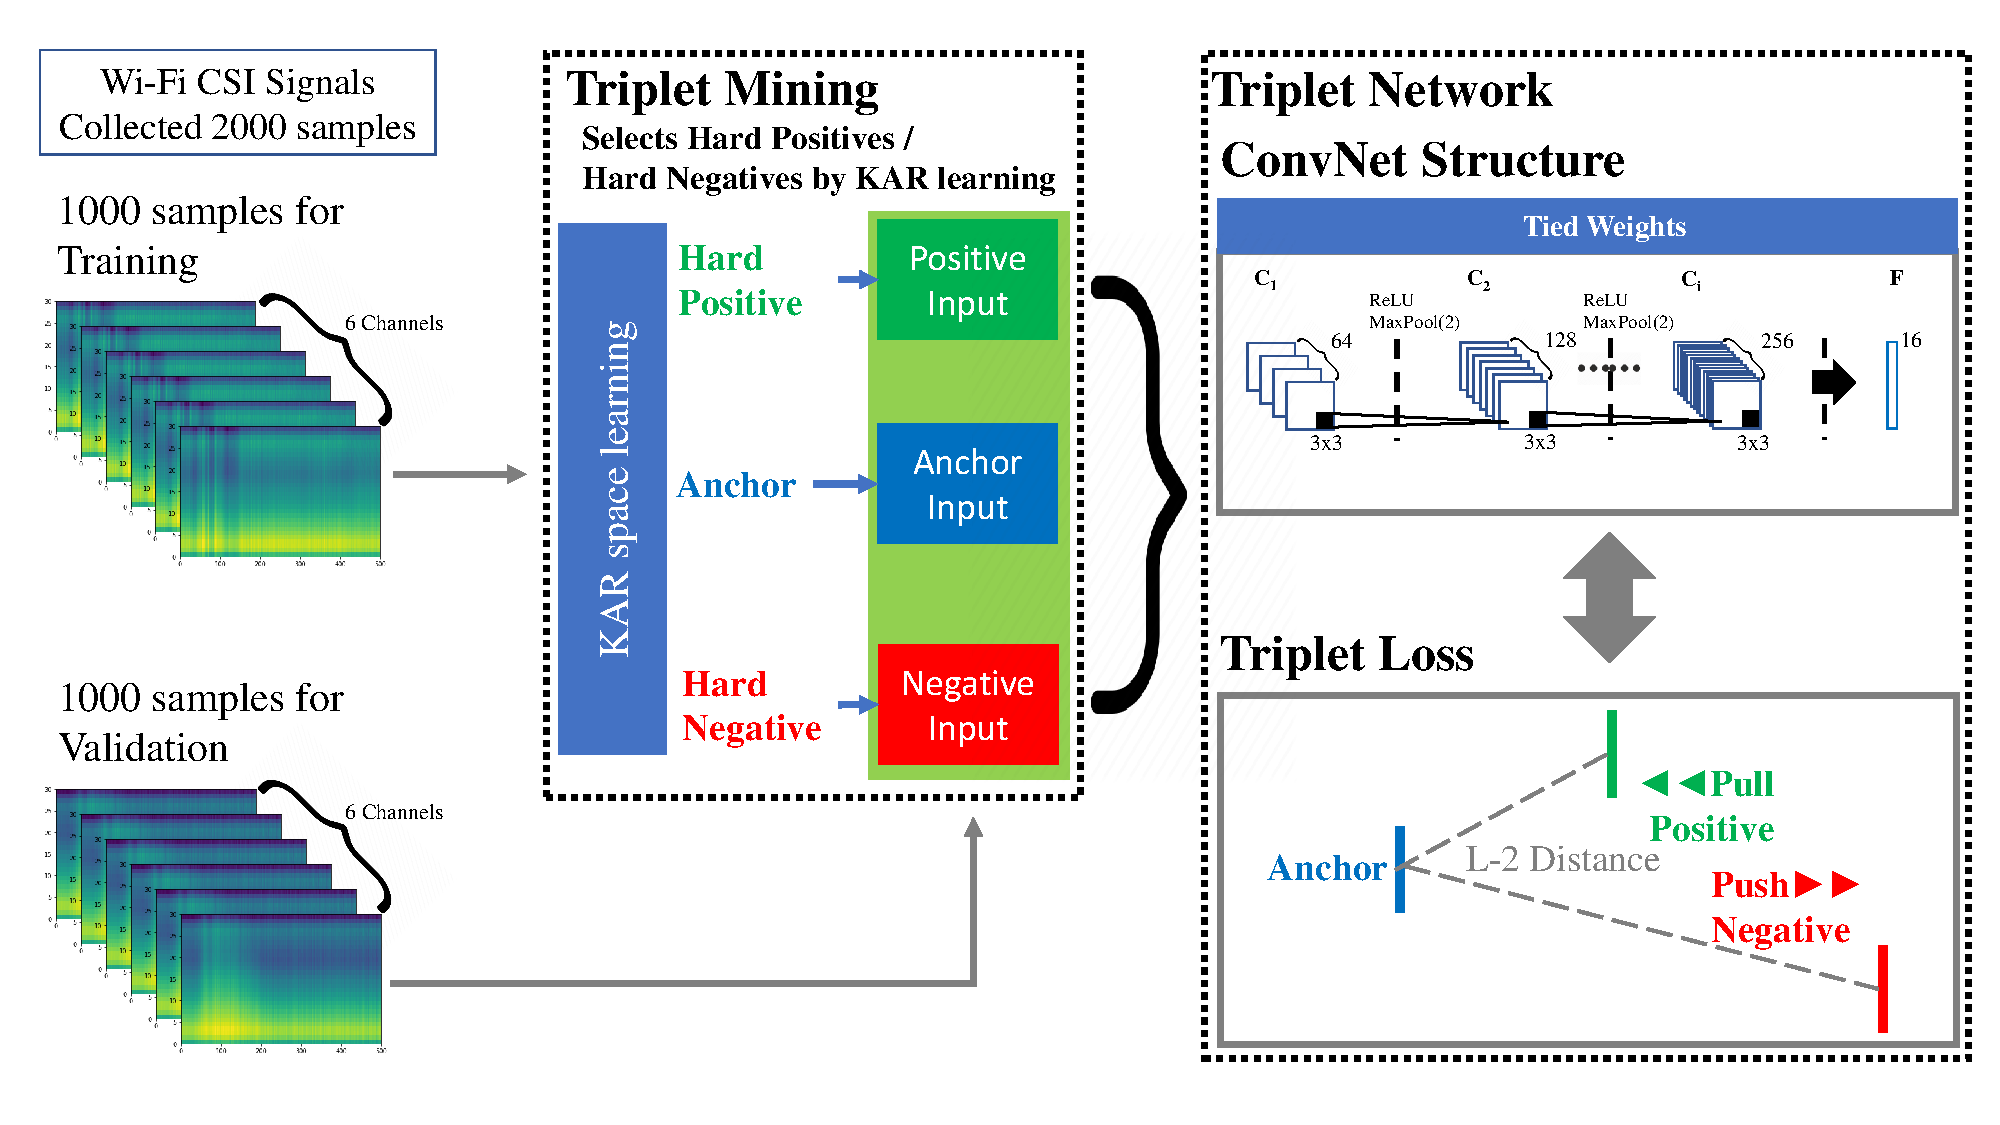
\includegraphics[width=\textwidth]{fig1_tcnn_kar_v2}
    \caption{Structure of the network} \label{fig1}
\end{figure}

% Methods: Triplet loss
\subsection{Triplet loss}

Triplet loss is used to train ConvNet to extract feature vector from triplet input.
For the $i_{th}$ anchor input signal $\mathbf{X}_{anc,i}$, triplet input is generated by grouping the positive input signal $\mathbf{X}_{pos,i}$ drawn from the same identity with anchor signal and the negative input signal $\mathbf{X}_{neg,i}$ is chosen from the another identity with the anchor signal.
Generated triplet input $\left\{\mathbf{X}_{anc,i},\mathbf{X}_{pos,i},\mathbf{X}_{neg,i}\right\}$ is fed into the ConvNet structure one by one and respectively makes anchor, positive and negative feature vectors.

Let $\mathbf{v}_{anc,i}\in{\mathrm{R}}^{d\times1}$, $\mathbf{v}_{pos,i}\in{\mathrm{R}}^{d\times1}$ and $\mathbf{v}_{neg,i}\in{\mathrm{R}}^{d\times1}$ be three feature vectors extracted from the ConvNet structure. 
the triplet loss is calculated by comparing positive distance (L-2 distance from the anchor vector to the positive feature vector) and negative distance (L-2 distance from the anchor vector to the negative feature vector).
ConvNet is trained to maximize gap between positive distance to negative distance more than margin $\alpha$.
The triplet loss for the inputs can be calculated as follows:

\begin{equation}
    loss = \sum_i^N max\left({ \left[ {\left\| {{\mathbf{v}_{anc,i}} - {\mathbf{v}_{pos,i}}} \right\|_2^2} - {\left\| {{\mathbf{v}_{anc,i}} - {\mathbf{v}_{neg,i}}} \right\|_2^2}  + \alpha \right]}, 0 \right),
\end{equation} 

where N is size of the mini-batch.
Note that the triplet loss can down to 0 when the negative distance is bigger than the positive distance more than preset margin $\alpha$.
If we select proper triplet for training, we can avoid this problem and make the convergence of the loss function faster. 

% Methods: KAR learning
\subsection{Triplet mining by kernel and the range space learning}
According to \cite{schroff2015facenet}, it is important to take hard positive and hard negative sample for faster convergence of the loss when training triplet networks.
we adopted KAR space learnig methods to approximate the ConvNet structure and mine the hard positive and the hard negative samples from the training dataset.

% importance of selecting hard pos/neg
Hard positive sample means distance between feature vectors from positive signal to anchor signal is the greatest, while hard negative sample means distance between feature vectors from negative signal to anchor signal is the smallest.

% methods of KAR learning
Since we don't know which is the hard sample before training the network, we propose to train multilayer feedforward neural network to mine the hard positive and the hard negative from the traning dataset.
To train the multilayer neural network, we adopted the kernel and the range (KAR) space projection learning (see Section2.2 for details).
% Methods: ConvNets
\subsection{ConvNet Structures}

To design the proposed networks, we firstly need to select the feature extracting networks which convert the triplet data into a feature vector. In this work, we utilize the ConvNet structure \cite{lecun1998gradient} as a feature extractor since the three-dimensional data format of our preprocessed input signal can be regarded as an image data format with multiple channels. 

Our ConvNet structure (See Fig~\ref{fig1} (b)) for the network consists of $i$ convolutional layers $\mathbf{C}_{i}$ and one fully-connected layer $\mathbf{F}$. The number of convolutional filters to be trained in each layer is empirically chosen as $\{64, 128, ...,  2^{6+i}\}$, with fixed filter size of $3\times3$ and stride of 1. The Rectified Linear (ReLU) function as an activation function and the max-pooling layers are applied between each convolutional layers. The features from the last convolutional layer are directly flattened into a single vector.
We used the sigmoid activation at ConvNet output and L-2 normalize output vectors to prevent negative distance when calculating triplet loss.

%Since the networks utilize three ConvNet structures which ties the weights each other, noting here that three structures described in Fig~\ref{fig1} (b) are actually the same model.

\section{Experiments}

% Dataset
\subsubsection{Dataset}
 In order to evaluate the verification performance of proposed system, Wi-Fi CSI signature dataset from \cite{moon2017air} was used. Wi-Fi CSI dataset consists of 2000 Wi-Fi CSI signature signals (4 directions $\times$ 50 identities $\times$ 10 samples) each signal is size of (500 packets $\times$ 30 subcarriers $\times$ 6 antennas). Since the Wi-Fi signature signals in CSI packets in 2.4Ghz has firmware issues in their phase \cite{wang2015understanding}. we used only absolute value.

 % pre-processing
 Since every Wi-Fi signature signal has different data size, we firstly adopted the gradient operation with respect to the time instance to measure the short time energy. Data points with the highest short-time energy within the time period are then manually selected as the starting and the ending points of the in-air signature action. Subsequently, the Fast Fourier Transform based re-sampling method \cite{moon2017air} is implemented to unify the length of the signals. As a result, three-dimensional Wi-Fi signature signals with unified data size are obtained as the input of the ConvNet structure in the network.

\subsubsection{Experimental Settings}

\subsubsection{1) Performance Evaluation}
% performance evaluation
The porposed method is evaluated under comparision of the proposed method with other verification methods based on verification accuracy.
verification performance is compared with existing linear methods in literature such as LSE, SVM and TER. Moreover, proposed method is compared by ConvNet based Siamese networks,we used same ConvNet model for our proposed method and Siamese network.

% Evaluation protocols
Validation performance of the proposed and other linear deep learning methods were evaluated in terms of Equal Error Rates (EER, \%) averaged from five runs of two-fold cross-validation tests. 

\subsubsection{2) Network Structure}
 We impose a triplet loss as objective function on our classifier. This objective is combined with standard backpropagation algorithm.
 The structure of the ConvNet network is specified in Table \ref{tab1}. we train the network starting with a learning rate of 0.00001 via Cross Entropy loss with a mini-batch sized of 32. We optimize the loss by the Adam optimizer with L-2 penalty of 0.0002 except for output layer. Output layer is regularized with L-2 penalty of 0.0001.
 We initialized all network weights in the convolutional layers from a normal distribution with zero-mean and a standard deviation of 0.01. Biases were also initialized from a normal distribution of standard deviation of 0.01, but with 0.5 mean.
 Training is conduced with 2000 iterations, which set empirically.
 
 \begin{table}[]
    \caption{The structure of ConvNet}\label{tab1}
    \centering
    \begin{tabular}{|l|l|l|l|}
    \hline
    Layer     & Activation & Kernel / Stride & Input Size \\ \hline
    Conv 1    & ReLU       & 3x3x64 / 1      & 500x30x6   \\
    MaxPool 1 &            & 2x2 / 1         & 500x30x64  \\
    Conv 2    & ReLU       & 3x3x128 / 1     & 250x15x64 \\
    MaxPool 2 &            & 2x2 / 1         & 250x15x128 \\
    Conv 3    & ReLU       & 3x3x256 / 1     & 125x8x128  \\
    MaxPool 3 &            & 2x2 / 1         & 125x8x256  \\
    Dense     & Sigmoid    & 128             & 63x4x256   \\
    L-2 Norm  &            &                 & 1x1x128    \\
    Concat    &            &                 & 1x1x384    \\ \hline
    \end{tabular}
\end{table}

For KARnet trainied multilayer neural networks is shown below (Table \ref{tab2}), we set 2 layer and number of neurons are [1024,16]. initialized as uniform distribution over [0, 1).
Used arctangent as activation function.

\begin{table}[]
    \caption{The structure of KARnet}\label{tab2}
    \centering
    \begin{tabular}{|l|l|l|}
    \hline
    Layer   & Size     & Activation \\ \hline
    Input   & 500x30x6 &            \\
    Dense 1 & 1x1x1024 & ArcTan     \\
    Dense 2 & 1x1x128  & ArcTan     \\
    Output  & 1x1x50   &            \\ \hline
    \end{tabular}
\end{table}

\subsubsection{3) Parameter Settings}
For making triplet loss, 0.1 of alpha value is utilized for the proposed method.
we choose output vector size of 16.
For linear methods such as LSE,SVM and TER, we reduced dimension of input signal to 500x30, by averaging through subcarrier axis. Due to limitation of hardware memory.
For PCA-LSE, input dimension is reduced by 40 sized features using PCA.
For Triplet CNN without KAR learning, we choose signature randomly for making input triplets and used triplet loss as used in proposed methods.
for Siamese Networks, we put 2 random signal as input and used binary loss for training the networks.

\subsubsection{Results and Discussion}

Table \ref{tab3} shows the best average EER performances obtained by the compared methods. The test EER was averaged from five runs of two-fold cross-validation.
Comparing with ConvNet based Siamese and Triplet CNN without KAR learning, proposed methods showed the best EER performance. Due to negative mining process included in making triplet loss.
The proposed method showed much better EER than linear methods, such as SVM,LSE and TER. Since linear methods use reduced input signal.

% Loss Curve
Loss curves of proposed method are shown in Fig.\ref{fig2}.
This shows that KAR learning not only helps ConvNet to train faster, but also makes it to extract better features. As the proposed method shows steeper loss curve when training, and the variance of the validation loss is smaller.

\begin{table}[]
    \caption{Verification Performance}\label{tab3}
    \centering
    \begin{tabular}{|l|l|l|}
    \hline
    Methology   &   Best EER (\%) &   Condition   \\  \hline
    Proposed(TripletCNN with KAR learning) &   19.09   &   lr=0.00005, alpha=0.1  \\
    Triplet CNN without KAR learning    &   20.08   &   lr=0.00005, alpha=0.1  \\
    Siamese CNN  &   24.09   &   lr=0.00005, alpha=0.1  \\
    SVM(RBF)    &   24.31   &   c=1, gamma=0.01/3000 \\
    SVM(Linear) &   28.23   &   c=1 \\
    LSE(Dimension Reduction by PCA)    &   30.79   &  40 dimension input    \\
    TER &   35.75   &   order=1   \\
    LSE &   48.44   &   \\  \hline
    \end{tabular}
\end{table}


% Figure 2
\begin{figure}
    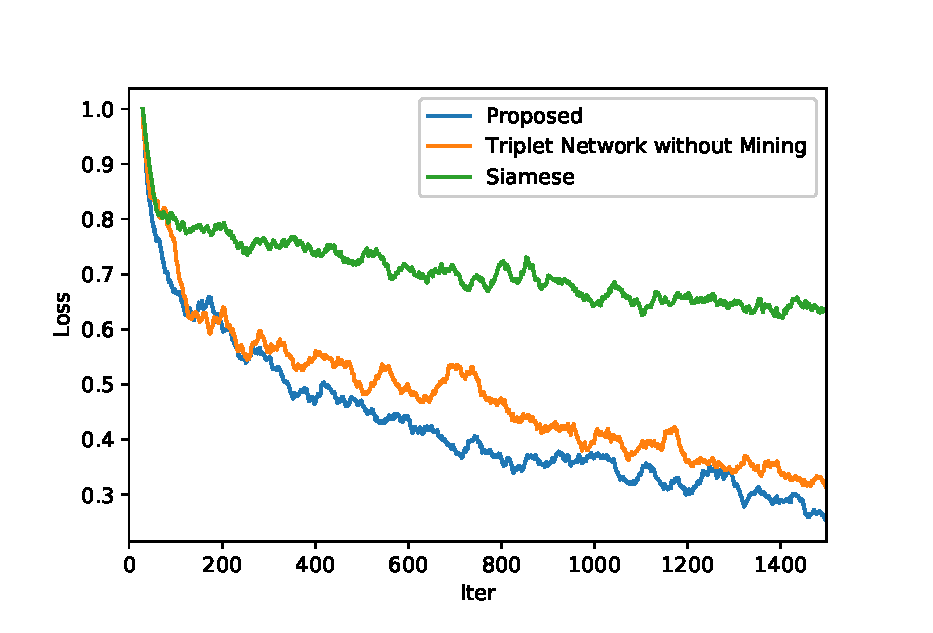
\includegraphics[width=\textwidth]{normalized_loss_curve_ma30.eps}
    \caption{Training Loss Curve of the Proposed Method} \label{fig2}
\end{figure}
% Figure 3
\begin{figure}
    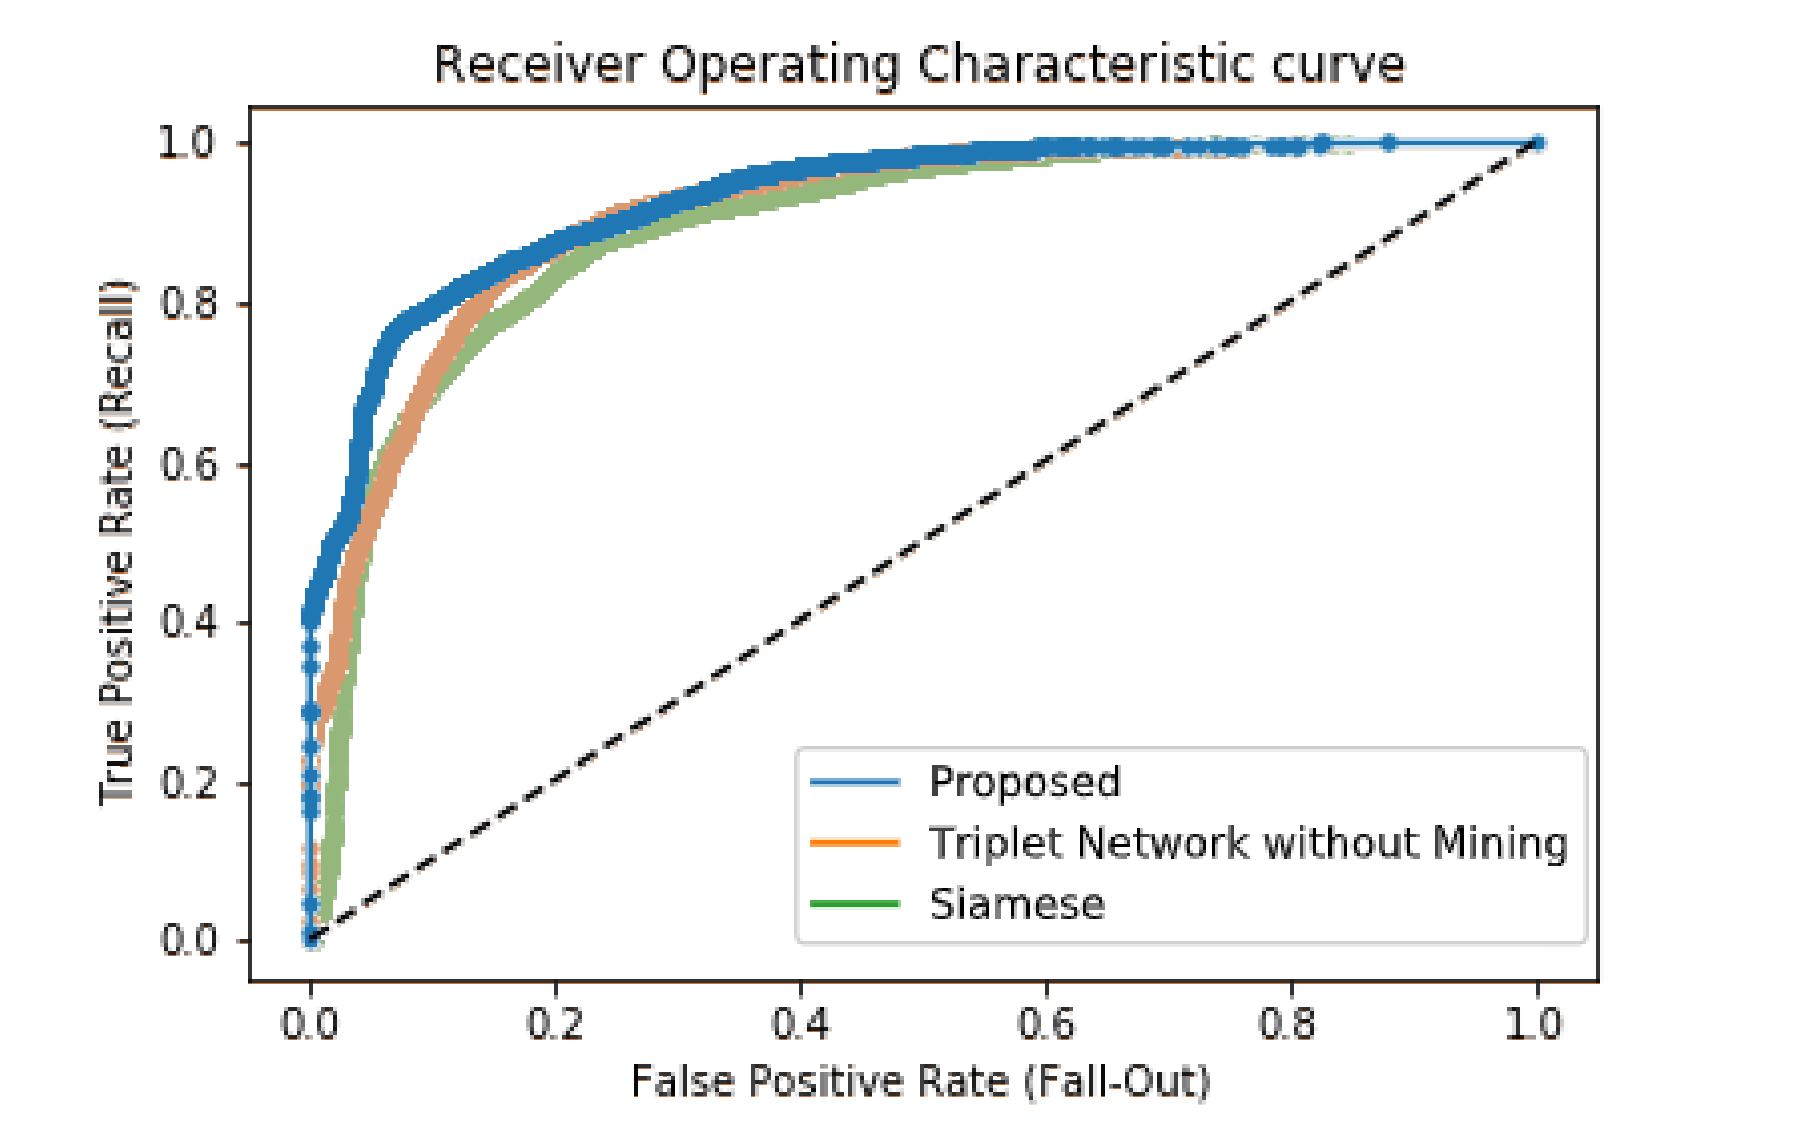
\includegraphics[width=\textwidth]{fig_roc.pdf}
    \caption{ROC Curve of the Proposed Method} \label{fig3}
\end{figure}

\section{Conclusion}
In this paper, we proposed a novel identity verification system based on Wi-Fi signature signals. 
In order to train the triplet network effectively, triplet input is mined from Wi-Fi signature signals by the kernel and the range space learning. Subsequently, ConvNet structure is adopted for feature extractor which generates feature vectors from input triplets. Finally, the triplet network is trained by matching between extracted feature vectors based on L-2 distance comparison. Our networks show good feature extracting performance, especially in low-dimension outputs and shows encouraging experimental results in terms of verification accuracy.
%
% ---- Bibliography ----
%
% BibTeX users should specify bibliography style 'splncs04'.
% References will then be sorted and formatted in the correct style.
%
%\bibliographystyle{splncs04}
%\bibliography{mybibliography}
%


%\begin{thebibliography}{8}

\bibliographystyle{splncs04}
\bibliography{bib_acpr}

%\end{thebibliography}

\end{document}